\documentclass[russian, a4paper, 12pt]{article}
\usepackage[utf8]{inputenc}
\usepackage[russian]{babel}
\usepackage{setspace,amsmath}
\usepackage[left=20mm, top=15mm, right=15mm, bottom=15mm, nohead, footskip=10mm]{geometry} % настройки полей документа
\usepackage{tocloft}
\usepackage{hyperref}
\hypersetup{
    colorlinks,
    citecolor=black,
    filecolor=black,
    linkcolor=black,
    urlcolor=black
}

%%% Работа с русским языком
\usepackage{cmap}					% поиск в PDF
\usepackage{mathtext} 				% русские буквы в формулах
\usepackage[T2A]{fontenc}			% кодировка
\usepackage[utf8]{inputenc}			% кодировка исходного текста
% \usepackage[english,russian]{babel}	% локализация и переносы

%%% Дополнительная работа с математикой
\usepackage{amsmath,amsfonts,amssymb,amsthm,mathtools} % AMS
\usepackage{icomma} % "Умная" запятая: $0,2$ --- число, $0, 2$ --- перечисление

%% Номера формул
\mathtoolsset{showonlyrefs=true} % Показывать номера только у тех формул, на которые есть \eqref{} в тексте.

%% Шрифты
\usepackage{euscript}	 % Шрифт Евклид
\usepackage{mathrsfs} % Красивый матшрифт


%% Перенос знаков в формулах (по Львовскому)
\newcommand*{\hm}[1]{#1\nobreak\discretionary{}
{\hbox{$\mathsurround=0pt #1$}}{}}
\renewcommand{\cftpartleader}{\cftdotfill{\cftdotsep}} % for parts
% \renewcommand{\cftchapleader}{\cftdotfill{\cftdotsep}} % for chapters
\renewcommand{\cftsecleader}{\cftdotfill{\cftdotsep}}
\begin{document} % начало документа
\begingroup
    \fontsize{14pt}{14pt}\selectfont
% НАЧАЛО ТИТУЛЬНОГО ЛИСТА
\begin{center}
\hfill \break
\footnotesize{НАЦИОНАЛЬНЫЙ ИССЛЕДОВАТЕЛЬСКИЙ УНИВЕРСИТЕТ}\\
\small{\textbf{«ВЫСШАЯ ШКОЛА ЭКОНОМИКИ»}}\\
\hfill \break
\normalsize{Факультет Компьютерных Наук}\\
 \hfill \break
\normalsize{Департамент Программной Инженерии}\\
\hfill\break
\hfill \break
\hfill \break
\hfill \break
\hfill \break
\hfill \break
\hfill \break
\hfill \break
\normalsize{Контрольное Домашнее Задание\\
\hfill \break
по дисциплине «Алгоритмы и Структуры Данных»\\
\hfill \break
\textbf{ОТЧЕТ}}\\
\hfill \break
\hfill \break
\end{center}

\hfill \break
\hfill \break
\hfill \break
\hfill \break
\begin{flushright}
  \normalsize{Выполнил:}\\
  \normalsize{Студент 2 курса группы БПИ151}\\
  \normalsize{Куприрянов Кирилл Игорвеич}
\end{flushright}
\hfill \break
\hfill \break
\hfill \break
\hfill \break
\hfill \break
\hfill \break
\hfill \break
\hfill \break
\hfill \break
\hfill \break
\hfill \break
\hfill \break
\hfill \break
\hfill \break
\hfill \break
\begin{center} Москва 2016 \end{center}
\thispagestyle{empty} % выключаем отображение номера для этой страницы

% КОНЕЦ ТИТУЛЬНОГО ЛИСТА
\endgroup

\newpage
    \tableofcontents % Вывод содержания
\newpage

\newpage
\section{Постановка задачи}
Необходимо было реализовать с использованием языка $C++$ программы для
архивирования и текстовых файлов. При этом использовать два известных алгоритма
кодирования информации:

\begin{enumerate}
  \item Хаффмана (не адаптивный, простой)
  \item Шеннона-Фано
\end{enumerate}
Обе реализации поместить в одном файле main.cpp, содержащем соответствующие методы:
\begin{enumerate}
  \item метод архивирования, использующий алгоритм Хаффмана,
  вход: текстовый файл <name>.txt (кодировка UTF-8)
  выход: архивированный файл <name>.haff
  \item метод разархивирования, использующий алгоритм Хаффмана,
  вход: архивированный файл <name>.haff
  выход: разархивированный файл <name>-unz-h.txt (кодировка UTF-8)
  \item метод архивирования, использующий алгоритм Шеннона-Фано,
  вход: текстовый файл <name>.txt (кодировка UTF-8)
  выход: архивированный файл <name>.shan
  \item метод разархивирования, использующий алгоритм Шеннона-Фано.
  вход: архивированный файл <name>.shan
  выход: разархивированный файл <name>-unz-s.txt (кодировка UTF-8)
\end{enumerate}

Выбор алгоритма осуществляется с помощью флага командной строки.

Оба алгоритма работают в два прохода. Сначала строится таблица частот
встречаемости символов в конкретном архивируемом файле (кодируем только те
символы из набора допустимых, которые реально встречаются в файле).
Затем строится кодовое дерево (не обязательное).
По нему (или по таблице кодов) и архивируется файл. Для
разархивирования алгоритмам потребуется знать таблицу, которая использовалась
при архивировании. Соответствующая таблица должна сохраняться в архивном файле
в самом его начале и использоваться при разархивировании. В начале пишется
количество различных символов n, имеющихся в кодируемом файле, а затем n пар (код
символа UTF-8, битовый код в архиве). Порядок — по убыванию частоты встречаемости
символа в кодируемом файле.

Провести вычислительный эксперимент с целью оценки реализованных
алгоритмов архивации / разархивации. Оценить количество элементарных операций
каждого алгоритма.
Для этого
\begin{enumerate}
  \item Подготовить тестовый набор из нескольких текстовых файлов разного объема
  (20, 40, 60, 80, 100 Кб; 1, 2, 3 Мб — всего 8 файлов) на разных языках (ru, en -
  кодировка UTF-8) с разным набором символов в каждом файле, а именно:
  \begin{enumerate}
    \item первый набор: символы латинского алфавита и пробел
    \item второй набор: символы из первого набора + символы русского алфавита
    \item третий набор: символы из второго набора + следующие знаки и
    спецсимволы: знаки арифметики „+ - * / =“, знаки препинания „. , ; : ? !“,
    „\% @ \# \$ \& ~‘’, скобки разных типов „( ) [ ] { } < >“ , кавычки „„““),
  \end{enumerate}
  \item Измерить (экспериментально) количество операций (в рамках модели RAM (взять из
    лекционного материала)), выполняемых за время работы (архивирования,
    разархивирования) каждого алгоритма на нескольких различных (не менее
    трех) файлах для каждого размера входного файла и набора символов (итого
    получается $8\times3\times3 = 72$ эксперимента по архивированию и 72 по
    разархивированию для каждого алгоритма, т.е. Всего минимум $144\times2 = 288$).
    Для повышения достоверности результатов каждый эксперимент можно повторить
    несколько (5-10) раз на файлах (с одним возможным набором символов) одного размера с
    последующим усреднением результата.
\end{enumerate}

Подготовить отчет по итогам работы, содержащий постановку задачи, описание
алгоритмов и задействованных структур данных, описание реализации, обобщенные
результаты измерения эффективности алгоритмов, описание использованных
инструментов (например, если использовались скрипты автоматизации), выводы о
соответствии результатов экспериментальной проверки с теоретическими оценками
эффективности исследуемых алгоритмов.
Отчет также должен содержать измерения качества архивации (степень сжатия =
отношение размеров выходного и входного файлов), оценку связи между степенью
сжатия для различных входных файлов (как влияют объем, язык, набор символов, их
разнообразие?) и временем работы (количеством операций) для каждого алгоритма.

\textit{Было выполнено: } Всё. + построены дополнительные графики
\newpage
\section{Описание алгоритмов и использованных СД}
\subsection{Для решения задачи алгоритмом Хаффмана}

\subsubsection{Структуры данных}
Для реализации архивирования - деархивирования алгоритмом Хаффмана я использовал
следующие \textbf{структуры данных}:
\begin{itemize}
  \item \textbf{Бинарное дерево} с узлами - указателями на объекты класса Node.
  Для их хранения использовался двусвязный список.
  \item \textbf{map <char, int>} - для хранения таблицы частот
  \item \textbf{map <char, vector<bool> >} - для хранения таблицы вида <<символ - его код>>
\end{itemize}

\subsubsection{Алгоритмы и функции}
Описание использованных \textbf{алгоритмов}

Использовались следующие функции:
\begin{itemize}
  \item \textbf{vector<char> getSymbols(string)} - для заполнения вектора
  символов символами из файла.
  По указанному пути файла создает поток и считывает все символы в вектор.
  Затем удаляет (делает push\_back) последний элемент - константу EOF,
  поскольку она лишняя. Сложность - $O(n)$
  \item \textbf{map<char, int> getFreq(vector<char>)} - для составления таблицы частот.
  По данному вектору символов составляет map<char, int> - где каждому символу ставится
  в соответствие его частота появления в данном вектре
  \item \textbf{void buildTree(map<char, int>)} - для построения дерева.
  Создает list<Node *> для содержания узлов деревьев. Изначально каждый Node
  в списке имеет значение с = char из входной map, n = частоте появления (значение int во входной map).
  Указатели на левых и правых детей равны $nullptr$. Процедура построения дерева происходит следующем образом:
  Список сортируется по возрастанию частоты появления символов (для этого использую
  функцию sort и структуру Compare, где перегружаю оператор ()).
  Затем берутся первые 2 элемента списка, они становятся детьми нового узла,
  который кладется в начало списка, а 2 прошлых - удаляются. Эта процедура происходит
  рекурсивно до тех пор, пока не останется в списке только 1 элемент - корень. Сложность - $O(n)$
  \item \textbf{void buildTable(Node*)} - для построения таблицы кодов, используя
  дерево. Начиная с корня, идем по дереву налево. Если
  левый ребенок не равен nullptr, добавляем во временный вектор code 0 и
  вызываем эту функцию, передавая в качетве аргумента указатель на этого ребенка.
  Аналогично с правым ребенком, только добавляем в вектор code не 0, а 1. Если же
  и левуй и правый дети - nullptr, то мы считаем, что вектор code представляет собой
  код символа, который находится в текущем узле и записываем это соответствие в map <char, vector <bool> >
  \item \textbf{void encodeHuff(string , string)} - для <<архивации>> файла.
  Архивация проиходит следующим образом. Открываю потоки ввода
  и вывода. Для потока вывода ставлю флаги - std::ios::binary, и std::ios::out,
  поскольку я буду писать в бинарный файл. Считываю все символы из входного файла
  в vector<char>, с помощью указанной выше функции. Записваю в выходной файл первым делом
  длину того вектра - количество символов в исходном файле. Это понадобится
  дальше при разархивировании. Затем составляю таблицу
  частот и вторым байтом записываю длину таблицы, другими словами, кол-во
  уникальных символов. Если эта длина равна еденице, значит,
  что исходный файл заполнен одним конкретным символом "первый байт" количество
  раз. В таком случае, мы его считываем и пишем его столько раз в выходной файл.
  При разархивировании это учитываем. Если же количество
  уникальных символов не равно 1, то продолжаем. Записываем таблицу соответствий
  сида <<символ - его частота>>. Затем строим дерево, таблицу кодов,
  проходимся по исходному файлу и выводим в архив
  код каждого символа следующим образом:

  Поскольку писать побитово нельзя, пишем побайтово. Аккумулируем биты в переменной
  buf и считаем сколько бит мы уже записали.
  Как только это количество станет равно 8, пишум buf в файл и обнуляем его.
  В конце, если у нас кол-во бито оказалось не кратным 8,
  пишум то, что осталось для того, чтобы заполнить недостающие биты.
  НЕ считать лишнего при разархивировании нам поможет первый байт -
  кол-во символов в исходном сообщении.
  \item \textbf{void decodeHuff(string , string)} - для <<деархивации>> файла.
  Открываю потоки, считываю первый байт - кол-во символов. Если оно равно
  1, то считываю второй байт - сколько раз повторяется этот конкретный символ.
  Затем считываю этот символ и пишу в аутпут его такое
  количество раз. Если же первый байт не еденица, то идем дальше. Считываем
  длину таблицы частот и такое количество раз считываем
  следующие байты, попутно инициализируя таблицу частот. На основе этой таблицы
  строится дерево. Затем декодирую само сообщение.
  Считываю байт информации в char byte и смотрю на него побитово, если бит равен
  1, то иду по дереву направо, если 0, то налево.
  Когда дошел до листа, я дописываю в результирующую строку символ в листе.
  Когда просмотрел 8 битов, считывю новый.
  Затем, после того, как прочитал весь файл, записываю в аутпут результирующую
  строку, но не всю, а только такое количество символов,
  сколько я считал в начале.
\end{itemize}

\subsection{Для решения задачи алгоритмом Шеннона-Фано}
\subsubsection{Структуры данных}
Для реализации архивирования - деархивирования алгоритмом Шеннона-Фано я использовал
следующие \textbf{структуры данных}:
\begin{itemize}
  \item \textbf{struct node} - основная структура для работы с алгоритмом
  Шеннона-Фано с двумя полями - char ch (символ) и float p (его
  вероятность появления в тексте)
  \item \textbf{node *freqTable} - таблица вероятностей, представляет собой
  динамический массив из элементов node
  \item \textbf{map<char, vector<bool> > table} - аналогичная (таблице кодов Хаффмана)
  таблица, которой каждому символу
  поставлен в соответствие его код
\end{itemize}

\subsubsection{Алгоритмы и функции}
Описание использованных \textbf{алгоритмов}

Использовались следующие функции:
\begin{itemize}
  \item \textbf{void shannonFano(int, int)} - функция, которая, собственно, выполняет
  процедуру Шеннона-Фано. Строит таблицу <<символ-код>>. Это рекрсивная функция. База:
  return, если в группе всего лишь 1 символ. Если 2 символа, первому добавляем к коду 0, а
  ко второму - 1. Для остальныйх вариантов: проходим по (отсортиированнной!) таблице, постепенно
  инкрементируя текущую сумму вероятностей до момента пока она не станет больше либо равной половине
  полной вероятности, а пока она меньше половины, мы на каждом шаге приписываем
  к коду текущего символа 0. Как только этот момент настал, добавляем к кодам тех элементов, что ниже 1.
  Рекурсивно вызываем функцию для первой и второй групп. Получили построенную таблицу кодов по алгориитму
  Шеннона-Фано.
  \item \textbf{void encodeSF(string, string)} - функция, идентичная аналогичной для кода Хаффмана.
  Длина сообщения записывается первым битом, кол-во уникальных символов - вторым, затем таблица соответствий
  символ - вероятность, затем само сообщение, так же, как и для алгоритма Хаффмана. Со случаем, когда длина
  таблицы = 1 разбираемся так же, как и там. Различие - в моей реализации задачи алгоритмом Шеннона-Фано
  \textit{не используется} дерево, используется лишь таблица кодов.
  \item \textbf{void decodeSF(string, string)} - функция, идентичная аналогичной для кода Хаффмана.
  После получения таблицы вероятностей, вызываю функцию shannonFano для построения таблицы кодов. По ней
  и декодируется сообщени, лежащее в последних байтах архива. Как только получаем новый битик,
  добавляем его во временный vector<bool> и по мере добавления, проверяю, есть ли он в таблице кодов
  с помощью функции isInTable. Если он там есть, ищу символ, соответствующий этому коду при помощи
  функции getchar.
  % Вот эти 2 прохода по все таблице при каждом получении всего лишь одного бита
  % сильно увеличивают всремя выполнения программы
  \item \textbf{char getchar(vector<bool>)} - вспомогательная функция. Возвращает символ, которому
  в таблице кодов соответствует данный вектор или 0, если такого нет.
\end{itemize}
\newpage
\section{Описание плана эксперимента}
План эксперимента состоит в следующем:
\begin{itemize}
  \item Сгенерировать набор тестоых файлов
  \item Запустить программу на них, подсчитав количество операций, и получив таблицу
  \item По полученной таблице построить графики
  \item Проанализировать результаты эксперимента
\end{itemize}


Для начала нужно сгенерировать тестовый набор из файлов разных размеров
(20, 40, 60, 80, 100 Кб, 1, 2, 3 Мб) и разных наборов символов,
каждого по три штуки, итого $8\times3\times3 = 72$ файла. Для генерации тестового набора
файлов будет написан скрипт на языке Python.

Для подсчета количества операций при архивировании - деархивировании двумя алгоритмами
этих 72х файлов, я будет сделано следующее. Будет глобальная переменная, изначально равная $0$
\textbf{long numberOfOperations} и она будет инкрементироваться там, где необходимо подсчитать
действие за операцию. Вызов библиотечных функций будет считаться за одну операцию.
В конце выполнения программы это число выведится в отдельный файл.

Затем для подсчета операций при всех упомянутых выше действий, будет написан еще один
скрипт на языке Python. Он попутно формировать csv таблицу, записвая в нее данные о размере файлов,
количесве операций, используемом алгоритме, и т.д. (табл. 1)
\begin{center}
    \begin{tabular}{| l | l | l | l | l | l | l | l | l |}
    \hline
    name & old\_size & new\_size & operations & algo & set & action & num & size \\ \hline
    \end{tabular}\\
    \textit{Таблица 1.}
\end{center}

Для более удобного построения графиков нужно будет отфильтровать таблицу, усреднив количества
операций для трех дубликатов. Отфильтровка будет производится в тетрадке jupyter notebook
на языке Python, при помощи библиотек pandas и numpy.

Построение графиков будет проводиться в той же среде, при помощи библиотеки matplotlib.
\newpage
\section{Результаты эксперимента - таблицы и графики}

\subsection{Таблицы}
Ниже приведена часть отфильтрованной таблицы. Полная таблица представлена в файле filtered.csv.

\begin{tabular}{ | l | l | l | l | l | l | l | l | l | }
\hline
	name & old\_size & new\_size & operations & algo & set & action & num & size \\ \hline
	set\_100\_1\_1.haff & 77611 & 106509 & 1427272 & haff & 1 & d & 1 & 100 \\ \hline
	set\_100\_2\_1.haff & 76829 & 106512 & 1435777 & haff & 2 & d & 1 & 100 \\ \hline
	set\_100\_3\_1.haff & 83701 & 106510 & 1570388 & haff & 3 & d & 1 & 100 \\ \hline
	set\_1\_1\_1.haff & 732537 & 1007739 & 13462131 & haff & 1 & d & 1 & 1 \\ \hline
	set\_1\_2\_1.haff & 724456 & 1007782 & 13341756 & haff & 2 & d & 1 & 1 \\ \hline
	set\_1\_3\_1.haff & 785493 & 1007785 & 14406953 & haff & 3 & d & 1 & 1 \\ \hline
	set\_20\_1\_1.haff & 18098 & 24579 & 333718 & haff & 1 & d & 1 & 20 \\ \hline
	set\_20\_2\_1.haff & 18202 & 24582 & 356596 & haff & 2 & d & 1 & 20 \\ \hline
	set\_20\_3\_1.haff & 19873 & 24579 & 404576 & haff & 3 & d & 1 & 20 \\ \hline
	set\_2\_1\_1.haff & 1458962 & 2007285 & 26810733 & haff & 1 & d & 1 & 2 \\ \hline
	set\_2\_2\_1.haff & 1441710 & 2007381 & 26543748 & haff & 2 & d & 1 & 2 \\ \hline
	set\_2\_3\_1.haff & 1564668 & 2007370 & 28647416 & haff & 3 & d & 1 & 2 \\ \hline
	set\_3\_1\_1.haff & 2185326 & 3006831 & 40159281 & haff & 1 & d & 1 & 3 \\ \hline
	set\_3\_2\_1.haff & 2159711 & 3006951 & 39751799 & haff & 2 & d & 1 & 3 \\ \hline
	set\_3\_3\_1.haff & 2342968 & 3006948 & 42881756 & haff & 3 & d & 1 & 3 \\ \hline
	set\_40\_1\_1.haff & 30004 & 40965 & 552385 & haff & 1 & d & 1 & 40 \\ \hline
	set\_40\_2\_1.haff & 29949 & 40966 & 572777 & haff & 2 & d & 1 & 40 \\ \hline
	set\_40\_3\_1.haff & 32695 & 40967 & 638421 & haff & 3 & d & 1 & 40 \\ \hline
	set\_60\_1\_1.haff & 47860 & 65544 & 880456 & haff & 1 & d & 1 & 60 \\ \hline
	set\_60\_2\_1.haff & 47573 & 65547 & 896903 & haff & 2 & d & 1 & 60 \\ \hline
	set\_60\_3\_1.haff & 51786 & 65548 & 988454 & haff & 3 & d & 1 & 60 \\ \hline
	set\_80\_1\_1.haff & 59766 & 81930 & 1099230 & haff & 1 & d & 1 & 80 \\ \hline
	set\_80\_2\_1.haff & 59301 & 81931 & 1113272 & haff & 2 & d & 1 & 80 \\ \hline
	set\_80\_3\_1.haff & 64449 & 81932 & 1221124 & haff & 3 & d & 1 & 80 \\ \hline
	set\_100\_1\_1.shan & 77676 & 106509 & 1636177 & shan & 1 & d & 1 & 100 \\ \hline
	set\_100\_2\_1.shan & 77126 & 106512 & 1623705 & shan & 2 & d & 1 & 100 \\ \hline
	set\_100\_3\_1.shan & 83778 & 106510 & 1733023 & shan & 3 & d & 1 & 100 \\ \hline
	set\_1\_1\_1.shan & 732700 & 1007739 & 15475307 & shan & 1 & d & 1 & 1 \\ \hline
	set\_1\_2\_1.shan & 726084 & 1007782 & 15358870 & shan & 2 & d & 1 & 1 \\ \hline
	set\_1\_3\_1.shan & 785787 & 1007785 & 16375760 & shan & 3 & d & 1 & 1 \\ \hline
	set\_20\_1\_1.shan & 18130 & 24579 & 378189 & shan & 1 & d & 1 & 20 \\ \hline
	set\_20\_2\_1.shan & 18275 & 24582 & 376902 & shan & 2 & d & 1 & 20 \\ \hline
	set\_20\_3\_1.shan & 19900 & 24579 & 402449 & shan & 3 & d & 1 & 20 \\ \hline
	set\_2\_1\_1.shan & 1459177 & 2007285 & 30824264 & shan & 1 & d & 1 & 2 \\ \hline
	set\_2\_2\_1.shan & 1444790 & 2007381 & 30581392 & shan & 2 & d & 1 & 2 \\ \hline
	set\_2\_3\_1.shan & 1565095 & 2007370 & 32617358 & shan & 3 & d & 1 & 2 \\ \hline
	set\_3\_1\_1.shan & 2185690 & 3006831 & 46173351 & shan & 1 & d & 1 & 3 \\ \hline
	set\_3\_2\_1.shan & 2164260 & 3006951 & 45813148 & shan & 2 & d & 1 & 3 \\ \hline
	set\_3\_3\_1.shan & 2343503 & 3006948 & 48852992 & shan & 3 & d & 1 & 3 \\ \hline
	set\_40\_1\_1.shan & 30037 & 40965 & 629726 & shan & 1 & d & 1 & 40 \\ \hline
	set\_40\_2\_1.shan & 30069 & 40966 & 626671 & shan & 2 & d & 1 & 40 \\ \hline
  $\vdots$ & $\vdots$ & $\vdots$ & $\vdots$ & $\vdots$ & $\vdots$ & $\vdots$ & $\vdots$ & $\vdots$ \\ \hline
\end{tabular}
\newpage
Описание признаков:
\begin{itemize}
  \item \textbf{name}: имя файла, над которым будет производиться работа. Первая цифра -
  размер, вторая - набор символов, треться - номер дубликата, но, поскольку таблица
  уже отфильтрована, везде на месте третей цифры стоит 1
  \item \textbf{old\_size}: старый размер файла, до того, как над ним было совершено действие
  \item \textbf{new\_size}: новый размер файла, после того, как над ним было совершено действие
  \item \textbf{operations}: количество операций, призошедших при совершении действия
  \item \textbf{algo}: алгоритм, при помощи которого выполнялось действие
  \item \textbf{set}: номер набора символов, взят из названия
  \item \textbf{action}: действие, которое и совершалось над файлом (c - compress, d - decompress)
  \item \textbf{num}: номер дубликата, взят из названия
  \item \textbf{size}: размер файла, взят из названия
\end{itemize}

\subsection{Графики}
По приведенной таблицы были построены следующие графики (всего 8 + 12 + 2 = 22 шт.):
\begin{enumerate}
  \item Зависимость количества операций (ось OY) от размера файла (ось OX) и размера
        набора символов (цвет линии) для каждого алгоритма архивирования /
        разархивирования. Должно быть 2 (алгоритма) * 2 (арх/разарх) * 2 (малые и
        большие файлы отдельно) набора графиков, на каждом 3 кривые (для каждого
        набора символов свой цвет)
\item Зависимость количества операций (ось OY) от размера файла (ось OX), и
      используемого алгоритма (цвет линии) для каждого набора символов. Должно
      быть 3 (набора символов) * 2 (арх/разарх) * 2 (малые и большие файлы
      отдельно) набора графиков, на каждом 2 кривые (для каждого алгоритма)
\item Зависимость количества операций (ось OY) от размера набора символов (ось OX)
      на файлах максимального размера (3 Мб) для каждого алгоритма архивирования
      / разархивирования (цвет линии). Должно быть 2 (арх/разарх) набора графиков,
      на каждом 2 кривые (для каждого алгоритма)
\end{enumerate}
\subsubsection{Первый набор графиков}
\begin{center}
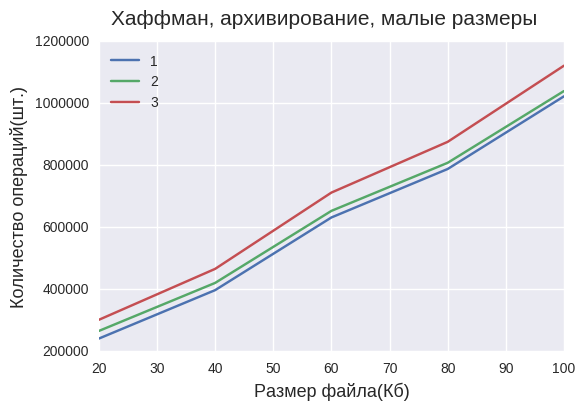
\includegraphics[width=0.9\linewidth]{./plots/1/1_1_1_1.png}\\
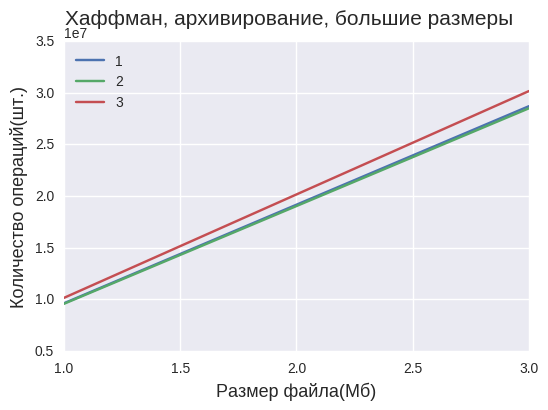
\includegraphics[width=0.9\linewidth]{./plots/1/1_1_1_2.png}\\
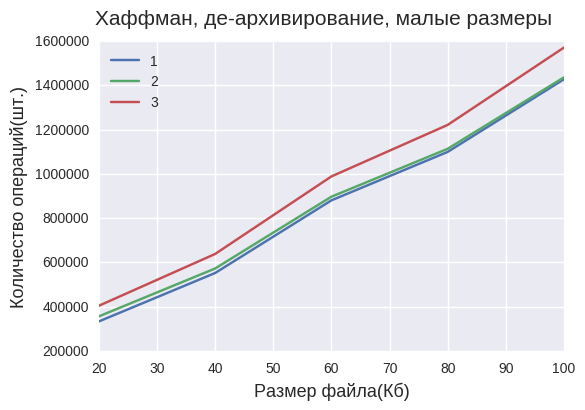
\includegraphics[width=0.9\linewidth]{./plots/1/1_1_2_1.png}\\
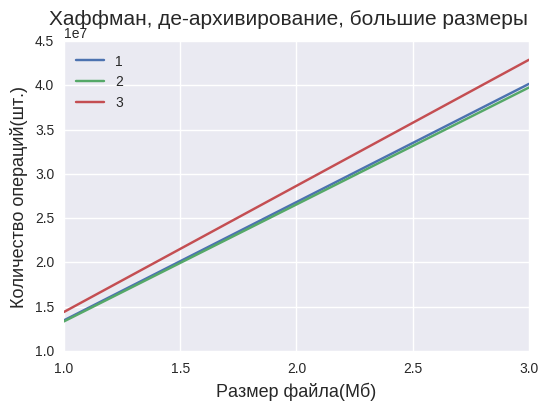
\includegraphics[width=0.9\linewidth]{./plots/1/1_1_2_2.png}\\
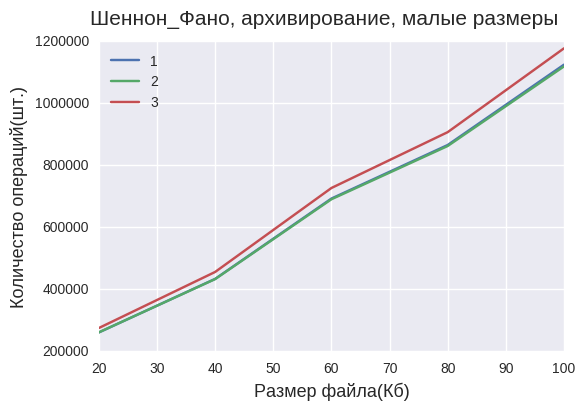
\includegraphics[width=0.9\linewidth]{./plots/1/1_2_1_1.png}\\
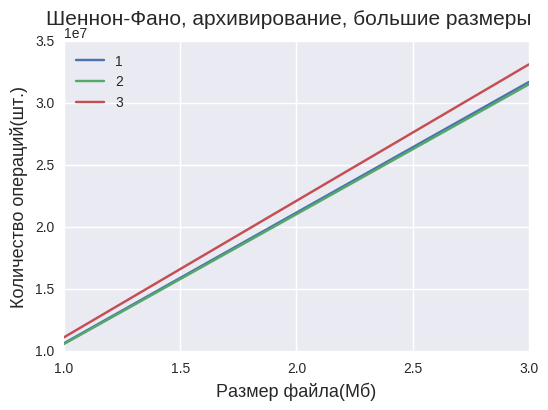
\includegraphics[width=0.9\linewidth]{./plots/1/1_2_1_2.png}\\
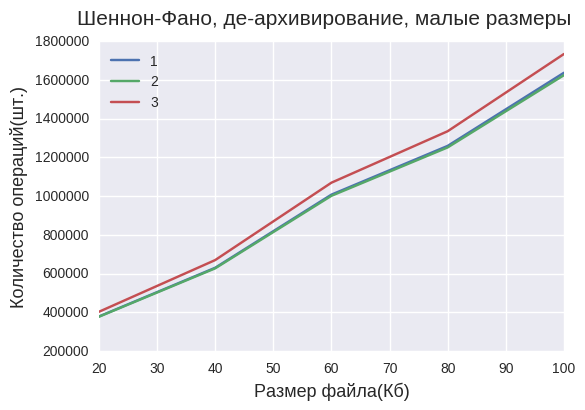
\includegraphics[width=0.9\linewidth]{./plots/1/1_2_2_1.png}\\
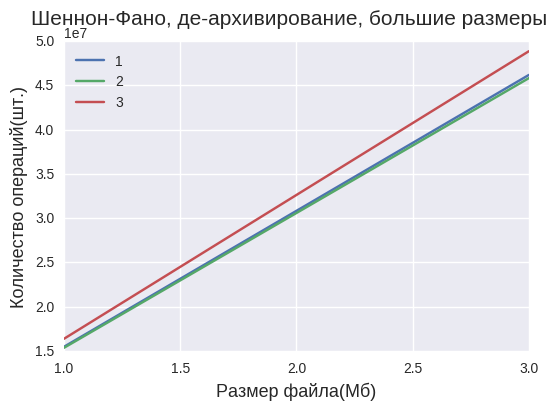
\includegraphics[width=0.9\linewidth]{./plots/1/1_2_2_2.png}\\
\end{center}

\subsubsection{Второй набор графиков}
\begin{center}
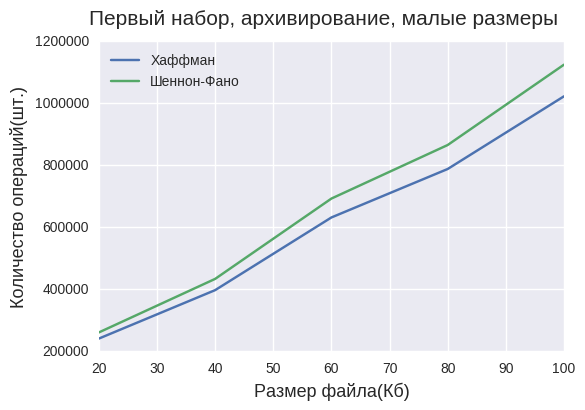
\includegraphics[width=0.9\linewidth]{./plots/2/2_1_1_1.png}\\
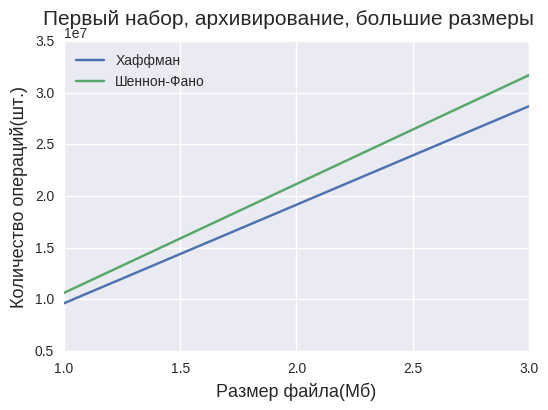
\includegraphics[width=0.9\linewidth]{./plots/2/2_1_1_2.png}\\
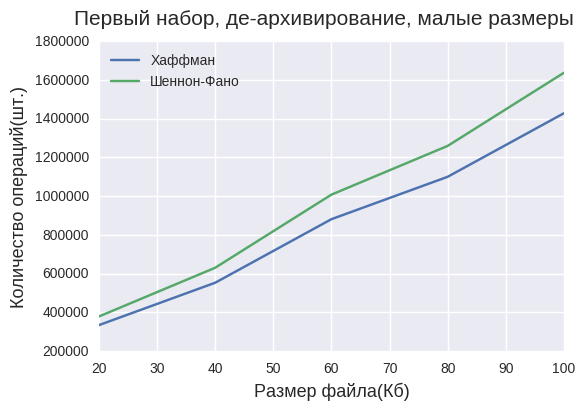
\includegraphics[width=0.9\linewidth]{./plots/2/2_1_2_1.png}\\
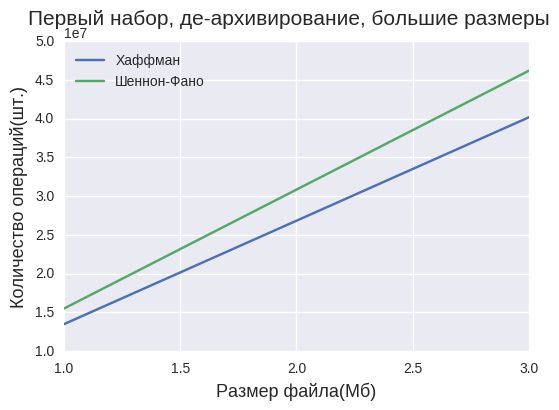
\includegraphics[width=0.9\linewidth]{./plots/2/2_1_2_2.png}\\
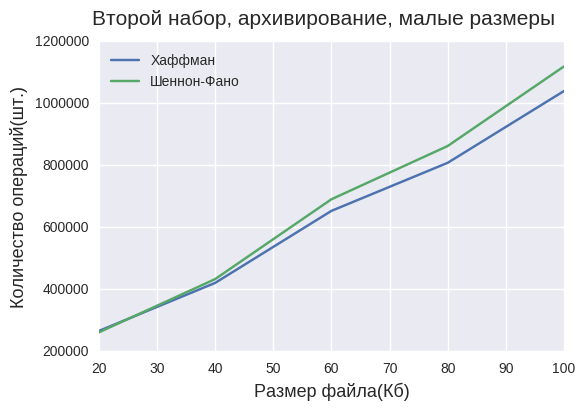
\includegraphics[width=0.9\linewidth]{./plots/2/2_2_1_1.png}\\
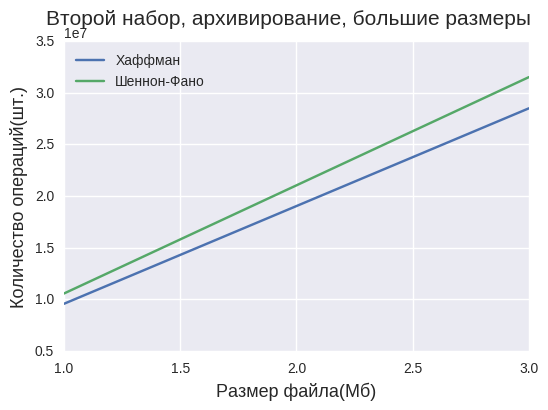
\includegraphics[width=0.9\linewidth]{./plots/2/2_2_1_2.png}\\
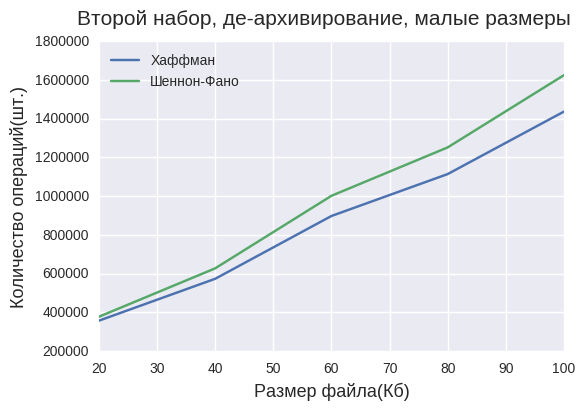
\includegraphics[width=0.9\linewidth]{./plots/2/2_2_2_1.png}\\
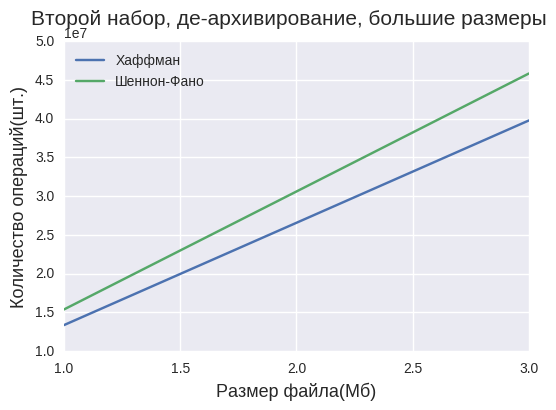
\includegraphics[width=0.9\linewidth]{./plots/2/2_2_2_2.png}\\
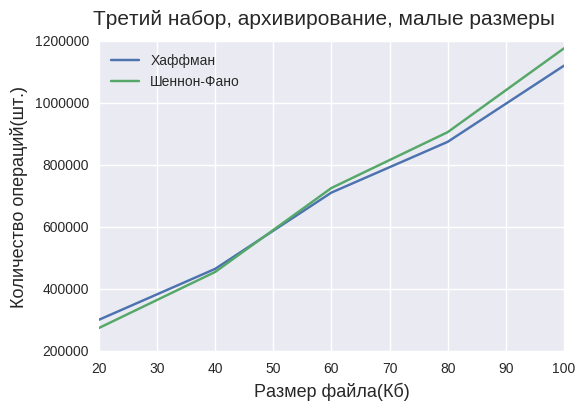
\includegraphics[width=0.9\linewidth]{./plots/2/2_3_1_1.png}\\
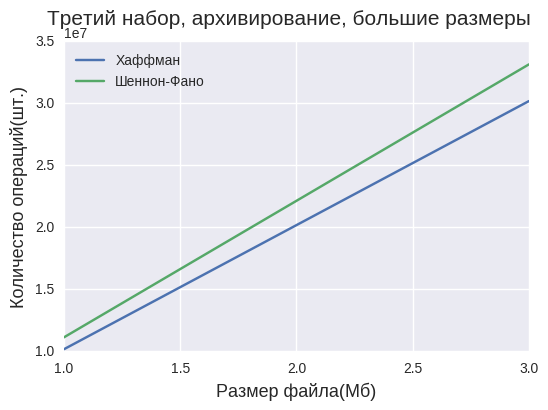
\includegraphics[width=0.9\linewidth]{./plots/2/2_3_1_2.png}\\
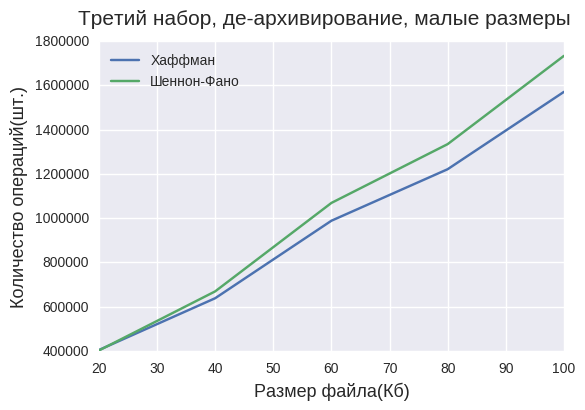
\includegraphics[width=0.9\linewidth]{./plots/2/2_3_2_1.png}\\
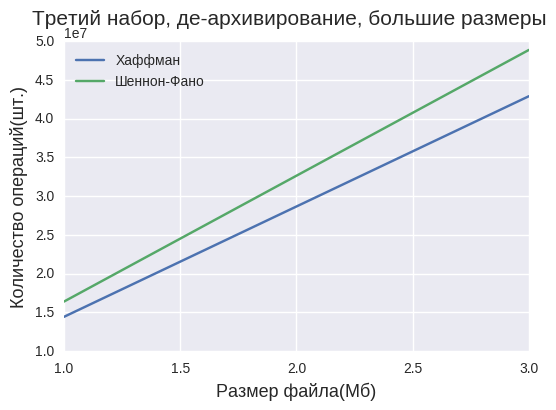
\includegraphics[width=0.9\linewidth]{./plots/2/2_3_2_2.png}\\
\end{center}

\subsubsection{Третий набор графиков}
\begin{center}
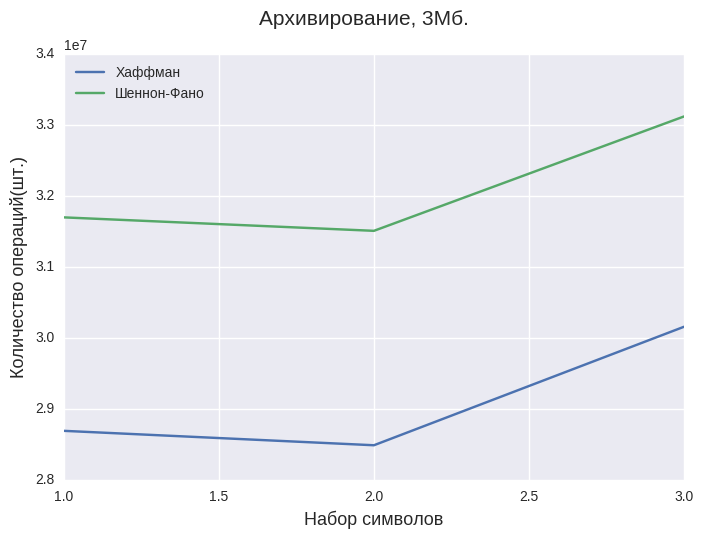
\includegraphics[width=0.9\linewidth]{./plots/3/3_1.png}\\
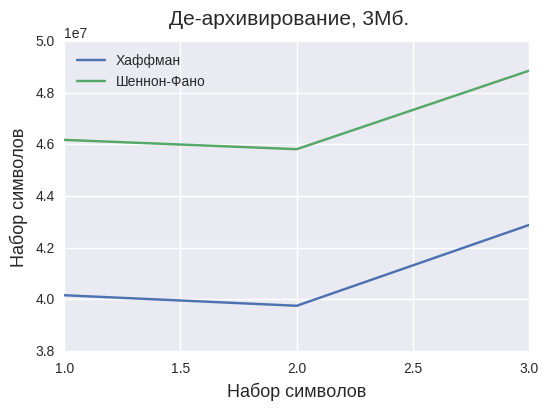
\includegraphics[width=0.9\linewidth]{./plots/3/3_2.png}\\
\end{center}

\newpage
По приведенным графикам видно, что архивирование - разархивирование
алгоритмом Хаффмана всегда занимает меньше операций, чем алгоритмом Шеннона-Фано.
Еще видно, что третий набор символов (со знаками пунктуаций, скобками, и т.д.) занимает
всегда больше операций, чем остальные, причем распределены они сответствующе. То есть
наименьшее кол-во операций требует архивация - деархивация файлов с английскими буквами,
пробелами и новыми строчками, затем тот же набор, но с русскими буквами, и на третьем месте
с символами. Единственное исключение - на третьем наборе графиков, когда на втором наборе кол-во
операций меньше, чем на первом.
\newpage
\subsection{Дополнительные графики}
Здесь приведены дополнительные графики, а именно, графики, иллюстрирующие степень сжатия файлов
в зависимости от используемого алгоритма, набора символов (цвет линии) и размера файлов.

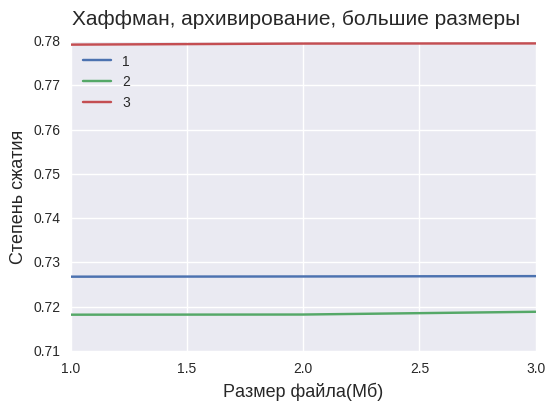
\includegraphics[width=0.9\linewidth]{./plots/additional/haff_arc_big.png}\\
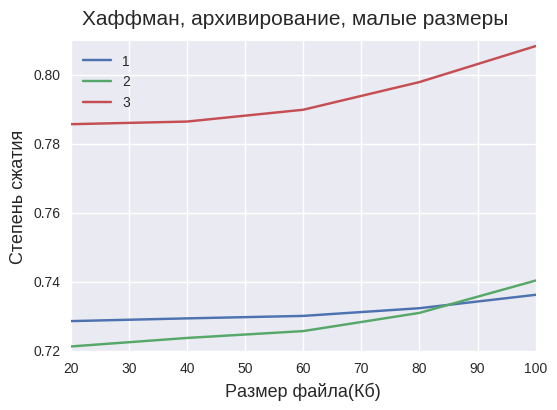
\includegraphics[width=0.9\linewidth]{./plots/additional/haff_arc_small.png}\\
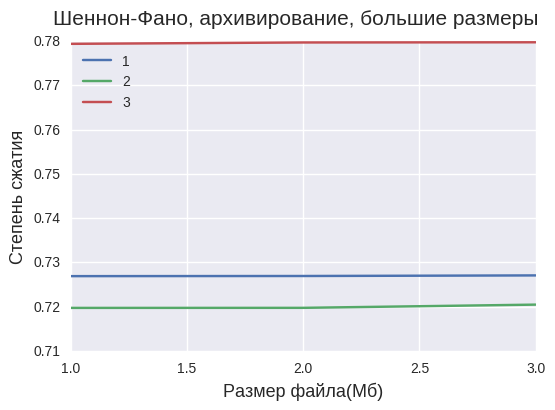
\includegraphics[width=0.9\linewidth]{./plots/additional/shan_arc_big.png}\\
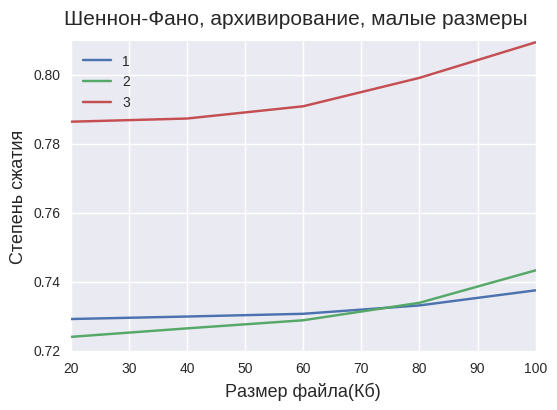
\includegraphics[width=0.9\linewidth]{./plots/additional/shan_arc_small.png}\\


Видно, что чем больше файл - тем больше степнь сжатия. Так же, файлы с третьим набором символов имеют
наибольшую степень сжатия. Интересно заметить, что при маленьких размерах файлов,
файлы со вторым набором символов и размером до 100 Кб имели меньшую степень сжатия алгоритмом
Хаффмана, чем файлы с первым набором символов. Аналогично с алгоритмом Шеннона-Фано, но только
для файлов до 80 Кб.
\newpage
\section{Сравнительный анализ методов}
Общее сравнение:

В моей реализации алгоритма Шеннона - Фано не использовалось дерево, в отличие от
реализации алгоритма Хаффмана. Следовательно, сложность его выше. Если не смотреть конкретно
на мою реализацию, то сложность будет примерно одинаковая. Оба алгоритма используют рекрсивные
функции для построения дерева, которые работают за $O(n)$.

Сравнение двух алгоритмов:

\begin{center}
    \begin{tabular}{ | p{8cm} | p{8cm} |}
    \hline
    \multicolumn{1}{|c|}{\textbf{Шеннон-Фано}} & \multicolumn{1}{|c|}{\textbf{Хаффман}} \\ \hline
    Дерево строится сверху-вниз & Дерево строится снизу-вверх\\ \hline
    Длина кодов в среднем большая & Длина кодов в среднем маленькая\\ \hline
    Легко реализуется & Немного сложнее реализуется\\ \hline
    Используемые СД: деревья, связные списки & Используемые СД: очереди с приоритетом, связные списки\\ \hline
    Нигде не используется & Используется при сжатии JPEG и mp3 файлов\\ \hline
    \end{tabular}
\end{center}
\section{Заключение}
В ходе работы над проектом была выполнена поставленная в начале задача. С использованием
языка C++ была написана программа для архивации и деархивации текстовых файлов. Были сгенерированы
тестовые текстовые файлы и проведены необходимые замеры. Составлена таблица, по ней построены
и проанализированы графики. Приводу основные выводы, к которым я пришел:
\begin{itemize}
  \item Степень и скорость сжатия лучше у алгоритма Хаффмана
  \item Алгоритм Хаффмана гарантирует построение кодов наименьей длины и наименьшим средним числом символов
  на букву при данном распределении вероятностей, в то время как алгоритм
  Шеннона - Фано не всегда приводит к однозначному построению кода.
  Дело в том, что на первой итерации функции ShannonFano, большей по сумме вероятностей
  може оказаться как первая, так и вторая половина набора. В результате среднее число
  символов на букву окажется другим. Таким образом, построенный код может оказаться не самым лучшим
  \item Алгоритм Хаффмана имеет повсеместное применение, используется присжатии изображений в формате JPEG/JPG,
  а так же для сжатия звука в формат mp3. Существует так же <<адаптивный алгоритм Хаффмана>>, который,
  считается лучше в некоторых случаях. Он работает в реальном времени, адаптируясь под текущую
  вероятность символов в кодируемом файле
  \item Для очень маленьких файлов степень сжатия может быть > 1, поскольку таблица частот,
  которая запишется в архив, может иметь такой размер, что в сумме с закодированным сообщением будет
  весить больше исходного текстового файла, не содежащего таблицу
\end{itemize}
\newpage
\section{Список используемых источников}
Литературные источники:

[1]  Кормен, Томас X., Лейзерсон, Чарльз И., Ривест, Рональд Л., Штайн, Клиффорд. Алгоритмы: построение
и анализ, 2-е издание.: Пер. с англ. М.: Издательский дом "Вильямc", 2005. ISBN 5-8459-0857-4. стр. 219,
стр. 459, стр. 216\\


Интернет - источники:

[2] Видеоурок "Алгоритм Хаффмана на С++":\\
https://www.youtube.com/watch?v=KNVPFVG49Oc Дата обращения: 27.11.2016

[3] Статья на википедии https://en.wikipedia.org/wiki/Huffman\_coding. Дата обращения: 30.11.2012

[4] Статья на википедии https://en.wikipedia.org/wiki/Shannon%E2%80%93Fano\_coding. Дата обращения: 1.12.2016
\end{document}
% EOF
